%\documentclass[13pt,handout]{beamer}
\documentclass[13pt]{beamer}
%\usetheme{Boadilla}

\usepackage[utf8]{inputenc}
\usepackage{tikz}
\usetikzlibrary{arrows,shapes}
\usepackage{graphicx}
\usepackage{gensymb}
\usepackage{verbatim}
\usepackage{multicol}
\usepackage[dutch]{babel}
\usepackage{dot2texi}

\usepackage{scalerel,fp}
\newlength\curht
\newlength\zshft
\newcounter{letcount}
\def\defaultdimfrac{.98}
\def\slantvalue{0}
\zshft=0pt\relax
\def\defaultstartht{\baselineskip}
\newcommand\diminish[2][\defaultdimfrac]{%
  \curht=\defaultstartht\relax
  \def\dimfrac{#1}%
  \setcounter{letcount}{0}
  \diminishhelpA{#2}%
}
\newcommand\diminishhelpA[1]{%
  \expandafter\diminishhelpB#1\relax%
}
\def\diminishhelpB#1#2\relax{%
  \FPpow\localshift{\dimfrac}{\theletcount}\unskip%
  \FPsub\localshift{1}{\localshift}%
  \FPsub\localdenom{1}{\dimfrac}%
  \FPdiv\localshift{\localshift}{\localdenom}%
  \raisebox{\localshift\zshft}{\scaleto{\strut\slantbox{#1}}{\curht}}%
  \stepcounter{letcount}%
  \curht=\dimfrac\curht\relax%
  \ifx\relax#2\relax\else\diminishhelpA{#2}\fi%
}
\newsavebox{\foobox}
\newcommand{\slantbox}[2][\slantvalue]{\mbox{%
    \sbox{\foobox}{#2}%
    \hskip\wd\foobox
    \pdfsave
    \pdfsetmatrix{1 0 #1 1}%
    \llap{\usebox{\foobox}}%
    \pdfrestore
  }}

% Set margins first argument left, second argument right
\def\changemargin#1#2{\list{}{\rightmargin#2\leftmargin#1}\item[]}
\let\endchangemargin=\endlist%

\title{Quiz}
\subtitle{Een wiskundige quiz}
\author{}
\institute{}
\date{}%\today}

\begin{document}

\begin{frame}
  \titlepage%
\end{frame}

% \begin{frame}
%   \frametitle{Outline}
%   \tableofcontents
% \end{frame}

\begin{frame}
  \frametitle{Vierkant}
  Hoeveel graden is de som van de hoeken van een vierkant?
  \vfill
  \begin{center}
    
\begin{tikzpicture}[scale=2,line cap=round,line
      join=round,>=triangle 45,x=1.0cm,y=1.0cm]
      \clip(-0.5,-0.5) rectangle (1.5,1.5); \filldraw[line
      width=1.6pt, fill=black,fill opacity=0.1] (0.,0.) -- (1.,0.) --
      (1.,1.) -- (0.,1.) -- cycle;
    \end{tikzpicture}
  \end{center}
  \vfill
  Antwoord: \uncover<2->{$4\cdot 90\degree=360\degree$}
\end{frame}

\newcommand\Num[2]{
  {\huge{#1}\small{#2}}
}

\begin{frame}
  \frametitle{Aanvullen}
  Wat zijn de laatste twee letters van onderstaande code
  \vfill
  \begin{changemargin}{-0.8cm}{-0.8cm}
    \begin{center}
      \Num{N}{\uncover<2->{ul}} \Num{E}{\uncover<3->{én}} \Num{T}{\uncover<4->{wee}} \Num{D}{\uncover<5->{rie}} \Num{V}{\uncover<5->{ier}} \Num{V}{\uncover<5->{ijf}} \Num{Z}{\uncover<5->{es}} \Num{Z}{\uncover<5->{even}} \Num{\_}{\uncover<6->{cht}} \Num{\_}{\uncover<6->{egen}}
    \end{center}
  \end{changemargin}
  \vfill
  Antwoord: {\uncover<6->{\Huge{A} \Huge{N}}}
\end{frame}

\begin{frame}
  \frametitle{Wollig}
  Welk dier bestaat voor $\dfrac{3}{4}$ uit wol?
  \vfill
  \begin{minipage}{0.45\linewidth}
    \uncover<2->{
      \begin{center}
        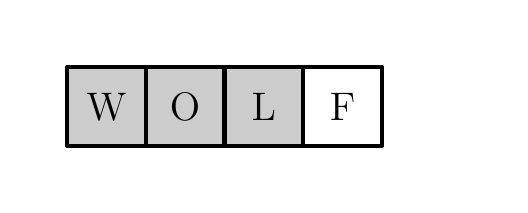
\begin{tikzpicture}[scale=1,line cap=round,line
          join=round,>=triangle 45,x=1.0cm,y=1.0cm]
          \clip(-0.5,-0.5) rectangle (5.5,1.5);
          \filldraw[line width=1.6pt, fill=black,fill opacity=0.2]
          (0,0) -- (1,0) -- (1,1) -- (0,1) -- cycle;
          \filldraw[line width=1.6pt, fill=black,fill opacity=0.2]
          (1,0) -- (2,0) -- (2,1) -- (1,1) -- cycle;
          \filldraw[line width=1.6pt, fill=black,fill opacity=0.2]
          (2,0) -- (3,0) -- (3,1) -- (2,1) -- cycle;
          \filldraw[line width=1.6pt, fill=black,fill opacity=0.0]
          (3,0) -- (4,0) -- (4,1) -- (3,1) -- cycle;
          \begin{Large}
            \uncover<3->{\draw (0.5,.5) node {W};}
            \uncover<4->{\draw (1.5,.5) node {O};}
            \uncover<4->{\draw (2.5,.5) node {L};}
            \uncover<5->{\draw (3.5,.5) node {F};}
          \end{Large}
        \end{tikzpicture}
      \end{center}
    }
  \end{minipage}
  \begin{minipage}{0.45\linewidth}
    \uncover<5->{
      \begin{center}
        % bron: https://www.clipartsfree.net/clipart/50604-wolf-backround-clipart.html
        \includegraphics[width=0.7\textwidth]{wolf}
      \end{center}
    }
  \end{minipage}
  \vfill
  Antwoord: \uncover<5->{Een wolf}
\end{frame}

\newcommand\clock[3][2]{%
\begin{tikzpicture}[scale=#1,line cap=round,line width=#1*3pt]
%\filldraw [fill=gray,transparent=0.5] (0,0) circle (2cm);
\foreach \angle / \label in
{0/3, 30/2, 60/1, 90/12, 120/11, 150/10, 180/9,
210/8, 240/7, 270/6, 300/5, 330/4}
{
\draw[line width=#1*1pt] (\angle:1.8cm) -- (\angle:2cm);
%\draw (\angle:1.4cm) node[scale=#1]{\textsf{\label}};
}
\foreach \angle in {0,90,180,270}
\draw[line width=#1*2pt] (\angle:1.6cm) -- (\angle:2cm);
\draw[rotate=90,line width=#1*2pt] (0,0) -- (-#2*30-#3*30/60:0.9cm); % hours
\draw[rotate=90,line width=#1*1.5pt] (0,0) -- (-#3*6:1.5cm); % minutes
\path [fill=black] (0,0) circle (3pt);
\path [fill=red] (0,0) circle (1.5pt);
%
\end{tikzpicture}%
}

\begin{frame}
  \frametitle{Mama eend}
  {\Large Mama eend en haar vijf kleintjes staan aan de rand van een $20$
  meter lange vijver. Aan de oever is er om de 4 meter een boom
  geplant. Hoelang doen de eendjes er over om de vijver over te
  zwemmen als je weet dat ze \alert<3>{een voor een} de vijver ingaan
  en \alert<3>{een na een} weer uit komen?}
  \vfill
  \uncover<2->{
  \begin{center}
    \alt<3->{\clock[0.8]{01}{01}}{\clock[0.8]{12}{59}}
  \end{center}
  }
  \vfill
  Antwoord: \uncover<3->{2 minuten!}
\end{frame}

\begin{frame}
  \frametitle{Priemgetallen}
  Wat is het kleinste priemgetal?
  \vfill
  \uncover<2->{
  \begin{definition}
    Een {\bf priemgetal} is een natuurlijk getal $>1$ dat juist twee
    natuurlijke getallen als deler heeft.
  \end{definition}
  }
  \vfill
  Antwoord: \uncover<3->{$2$}
\end{frame}

\begin{frame}
  \frametitle{Vul aan}
  Vul het volgende getal aan
  \[2 \qquad 3 \qquad 5 \qquad 7 \qquad 11 \qquad 13 \qquad 17 \qquad \ldots\]
  \vfill
  \uncover<2->{
  \begin{center}
    \vspace*{-1cm}
    \tikzset{
      number/.style={circle,inner sep=1pt},
      prime number/.style={number,fill=lime},
      non prime number/.style={number,fill=white,draw=red!50},
    }
    \begin{tikzpicture}[font=\bfseries\tiny,scale=0.7]
      \coordinate (last);
      \foreach \nb in {0,...,50}{
        \pgfmathsetmacro{\r}{sqrt(\nb)*.5}
        \pgfmathsetmacro{\a}{sqrt(\nb)*360}
        \coordinate(new) at (\a:\r);
        \draw[dotted] (last) to[bend right={6/sqrt(\nb)}] (new);
        \pgfmathisprime{\nb}
        \ifnum\pgfmathresult=0
        \node[non prime number](last) at (\a:\r) {\nb};
        \else
        \node[prime number](last) at (\a:\r) {\nb};
        \fi
      }
    \end{tikzpicture}
  \end{center}
  }
  \vfill
  \vspace*{-1cm}
  Antwoord: $\quad 2 \qquad 3 \qquad 5 \qquad 7 \qquad 11 \qquad 13
  \qquad 17 \qquad \alt<3>{\bf 19}{?}$
\end{frame}

\newcommand\parklot[1]{
  \begin{tikzpicture}
    [scale=0.4,rotate=#1,line cap=round,line join=round,>=triangle 45,x=1.0cm,y=1.0cm]
    \clip(-0.5,-0.5) rectangle (24.5,6.5);
    \draw [line width=1.6pt] (0.,0.)-- (0.,6.);
    \draw [line width=1.6pt] (4.,6.)-- (4.,0.);
    \draw [line width=1.6pt] (8.,6.)-- (8.,0.);
    \draw [line width=1.6pt] (11.6,6.)-- (11.6,0.);
    \draw [line width=1.6pt] (16.,6.)-- (16.,0.);
    \draw [line width=1.6pt] (20.,6.)-- (20.,0.);
    \draw [line width=1.6pt] (24.,6.)-- (24.,0.);
    \draw [line width=1.6pt] (0.,6.)-- (24.,6.);
    \draw (2,4.5) node[anchor=center, rotate=#1] {$86$};
    % bron: https://www.clipartsfree.net/clipart/36899-gray-car-top-view-270-clipart.html
    \node[rotate=#1] (car) at (6,2.75) {\includegraphics[width=1.15cm]{car}};
    \draw (10,4.5) node[anchor=center, rotate=#1] {$88$};
    \draw (14,4.5) node[anchor=center, rotate=#1] {$89$};
    \draw (18,4.5) node[anchor=center, rotate=#1] {$90$};
    \draw (22,4.5) node[anchor=center, rotate=#1] {9I};
  \end{tikzpicture}
}

\begin{frame}
  \frametitle{Parkeerplaats}
  Op welke parkeerplaats staat de auto?
  \vfill
  \begin{center}
    \alt<2->{\parklot{0}}{\parklot{180}}
  \end{center}
  \vfill
  Antwoord: \uncover<3->{Op plaats 87}
\end{frame}

\begin{frame}
  \frametitle{Machten}
  De meesten onder jullie kennen het programma twee tot de zesde
  macht, maar hoeveel is dit eigenlijk?  \vspace{0.5cm}

  \uncover<2->{ Als $a\in\mathbb{R}$ en $n\in\mathbb{N}_0$ dan wordt
    de $n$-de {\bf macht} van $a$ gedefinieerd als een product van $n$
    factoren van $a$:
  $$a^n=\underbrace{a\cdot a\cdot \cdots \cdot a}_{\text{$n$ factoren}}$$
  }
  \vfill
  Antwoord:
  \vspace{-2em}
  \uncover<3>{
  \begin{align*}
    2^6 &= 2\cdot2\cdot2\cdot2\cdot2\cdot2\\
        &= 2^3\cdot2^3\\
        &=8\cdot8\\
        &=64
  \end{align*}
  }
\end{frame}

\newcommand{\driekant}[4]{
  \begin{tikzpicture}
    [scale=0.23,rotate=60,line cap=round,line join=round,>=triangle 45,x=1.0cm,y=1.0cm]
    \clip(-1.5,-1.5) rectangle (9.5,9.5);
    \draw[line width=1.6pt,fill=black,fill opacity=0.05]
    (0.,0.) -- (8.,0.) -- (4.,6.9282032302755105) -- cycle;
    \draw (4,8.) node[anchor=center] {#1};
    \uncover<2->{\draw (6.8,3.9) node[anchor=center] {$+$};}
    \draw (8.9,0) node[anchor=center] {#2};
    \draw (-.9,0) node[anchor=center] {#3};
    \draw (4,2.6) node[anchor=center] {#4};
  \end{tikzpicture}
}

\begin{frame}
  \frametitle{Het rekenen verloopt driekant}
  Welk getal moet er worden ingevuld op de plaats van het vraagteken?
  \vfill
  \begin{changemargin}{-.8cm}{-.8cm}
      \begin{minipage}{0.24\textwidth}\driekant{13}{3}{8}{2}\end{minipage}
      \begin{minipage}{0.24\textwidth}\driekant{2}{4}{3}{2}\end{minipage}
      \begin{minipage}{0.24\textwidth}\driekant{2}{5}{1}{7}\end{minipage}
      \begin{minipage}{0.24\textwidth}\driekant{11}{5}{4}{?}\end{minipage}
  \end{changemargin}
  \vfill
  Antwoord: \quad\uncover<3->{$\dfrac{11+5}{4}=4$}
\end{frame}

\begin{frame}
  \frametitle{Juiste plaats}
  Onderstaande gelijkheid is vals:
   \[\scalebox{1.5}{$26-63=1$}\]
  Hoe kan je de gelijkheid waar maken door slechts één cijfer te verschuiven?
  \vfill
  \uncover<2->{
    {\color{blue} Een hint: Wiskunde bouwt verder op wat reeds gezien is. Wat weten we al uit voorgaande slides?}
  }
  \vfill
  Antwoord:  \uncover<3->{\[\scalebox{1.5}{$2^6-63=1$}\]}
\end{frame}

\begin{frame}
  \frametitle{Binair}
  {\scriptsize \em``Er zijn 10 soorten mensen:\\ Mensen die binair kunnen tellen en mensen die dat niet kunnen.''}\\
  \vfill
  Hoeveel is $20$ als decimaal getal binair geschreven?
  \vfill
  \uncover<2->{
  \begin{center}
    \begin{tabular}{c|ccccccc|c}
      \alt<2->{Binair & $2^3$ && $2^2$ && $2^1$ && $2^0$ & Decimaal}{&&&&&&&&}\\
      \hline
      \alt<2->{0000 & 0 & + & 0 & + & 0 & + & 0 & 0}{&&&&&&&&}\\
      \alt<3->{0001 & 0 & + & 0 & + & 0 & + & {\bf 1} & 1}{&&&&&&&&}\\
      \alt<4->{0010 & 0 & + & 0 & + & {\bf 2} & + & 0 & 2}{&&&&&&&&}\\
      \alt<5->{0011 & 0 & + & 0 & + & {\bf 2} & + & {\bf 1} & 3}{&&&&&&&&}\\
      \alt<6->{0100 & 0 & + & {\bf 4} & + & 0 & + & 0 & 4}{&&&&&&&&}\\
    \end{tabular}
  \end{center}
  }
  \vfill
  Antwoord: \uncover<7->{$20=16+4={\bf 1}\cdot 2^4 + {\bf 0}\cdot 2^3 + {\bf 1}\cdot 2^2 + {\bf 0}\cdot 2^1 + {\bf 0}\cdot 2^0=10100_2$}
\end{frame}



% \begin{frame}
%   \frametitle{Cirkel delen}
%   Op 10 oktober is het {\color{gray} S}tien haar $10$-de verjaardag. Ze wil haar verjaardagstaart in $10$ even grote stukken verdelen. Hoeveel keer moet zij minimaal snijden?
%   \vfill
%   \begin{center}
%     \definecolor{yqyqyq}{rgb}{0.5019607843137255,0.5019607843137255,0.5019607843137255}
%     \begin{tikzpicture}[scale=1.4,line cap=round,line join=round,>=triangle 45,x=1.0cm,y=1.0cm]
%       \clip(-1.4,-1.1) rectangle (1.4,1.3);
%       \draw [line width=2.pt] (0.,0.) circle (1.cm);
%       \uncover<2->{
%         \draw [line width=1.6pt,color=yqyqyq]
%         (0.,-1.3) -- (0.,1.3);
%       }
%       \uncover<3->{
%         \draw [line width=1.6pt,color=yqyqyq,domain=-1.3:1.3]
%         plot(\x,{(-0.--0.8090169943749475*\x)/0.5877852522924731});
%       }
%       \uncover<4->{
%         \draw [line width=1.6pt,color=yqyqyq,domain=-1.3:1.3]
%         plot(\x,{(-0.--0.30901699437494745*\x)/0.9510565162951536});
%       }
%       \uncover<5->{
%         \draw [line width=1.6pt,color=yqyqyq,domain=-1.3:1.3]
%         plot(\x,{(-0.-0.3090169943749474*\x)/0.9510565162951536});
%       }
%       \uncover<6->{
%         \draw [line width=1.6pt,color=yqyqyq,domain=-1.3:1.3]
%         plot(\x,{(-0.-0.8090169943749475*\x)/0.5877852522924731});
%       }
%       % \begin{scriptsize}
%       %   \draw [fill=black] (0.,0.) circle (1.0pt);
%       %   \draw[color=black] (-0.25,0.2) node {$A$};
%       %   \draw [fill=black] (0.,1.) circle (1.0pt);
%       %   \draw[color=black] (-0.13979728547401865,1.1917833206993669) node {$B$};
%       %   \draw [fill=black] (0.5877852522924731,0.8090169943749475) circle (1.0pt);
%       %   \draw[color=black] (0.6279478195912039,1.0317854624748377) node {$B'$};
%       %   \draw[color=black] (0.2,0.5) node {$36\degree$};
%       %   \draw [fill=black] (0.9510565162951536,0.30901699437494745) circle (1.0pt);
%       %   \draw[color=black] (1.159463661559435,0.48322137713359503) node {$B''$};
%       %   \draw [fill=black] (0.9510565162951536,-0.3090169943749474) circle (1.0pt);
%       %   \draw[color=black] (1.2893897562627803,-0.2824826586552229) node {$B'''$};
%       %   \draw [fill=black] (0.5877852522924731,-0.8090169943749475) circle (1.0pt);
%       %   \draw[color=black] (0.9,-0.8) node {$B''''$};
%       % \end{scriptsize}
%     \end{tikzpicture}
%   \end{center}
%   \vfill
%   Antwoord:
%   \uncover<7->{
%     Elke verdeling zorgt voor 2 extra stukken,
%     $$\Rightarrow 5 \text{ keer snijden}$$
%   }
% \end{frame}

\begin{frame}
  \frametitle{Balk}
  Hoeveel ribben heeft een balk?
  \uncover<2->{
    \begin{center}
      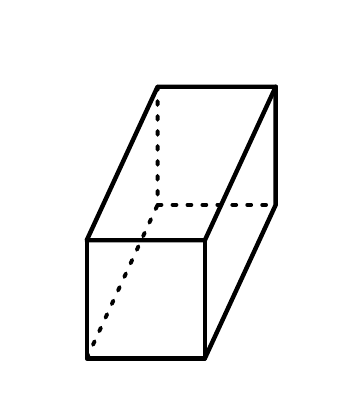
\begin{tikzpicture}[scale=1.5,line cap=round,line
        join=round,>=triangle 45,x=1.0cm,y=1.0cm]
        \clip(-0.5,-0.2) rectangle (2.1,2.8); \draw[line width=1.6pt]
        (0.,0.) -- (1.,0.) -- (1.,1.) -- (0.,1.) -- cycle; \draw[line
        width=1.6pt] (0,1) -- (0.6,2.3) -- (1.6,2.3) -- (1,1) -- cycle;
        \draw[line width=1.6pt] (1.6,2.3) -- (1.6,1.3) -- (1,0);
        \draw[line width=1.4pt,loosely dotted] (0,0) -- (0.6,1.3) --
        (0.6,2.3); \draw[line width=1.4pt,loosely dotted] (0.6,1.3) --
        (1.6,1.3);
      \end{tikzpicture}
    \end{center}
  }
  Antwoord:\\
  \uncover<3->{
    $6$ rechthoeken, elke rechthoek heeft $4$ zijden, elke zijde tweemaal geteld
    \[\Rightarrow 12 \mbox{ ribben}\]
  }
\end{frame}

\begin{frame}
  \frametitle{Loopwedstrijd}
  In een loopwedstrijd haal je de tweede loper in, op welke plaats loop je dan?
  \vfill
  \uncover<2->{
    \begin{center}
      % bron: https://www.clipartsfree.net/large/46421-runners-clipart.html
      \includegraphics[width=.8\textwidth]{lopers}
    \end{center}
  }
  Antwoord: \uncover<3->{$2$-de plaats}
\end{frame}

\begin{frame}
  \frametitle{Stelsel}
  Bereken:
  \begin{align*}
    \bigcirc + \bigcirc + \bigcirc &= 30\\
    \bigcirc + \square + \square &= 18\\
    \square - \bigtriangleup &= 2\\
    \bigtriangleup + \bigcirc \cdot \square &= \;?
  \end{align*}
  % \vfill

  \begin{scriptsize}
    \uncover<2->{
      \[\left\{
          \begin{aligned}
            3x &= 30\\ x + 2y   &= 18\\ y - z   &= 2\\ z + x\cdot y   &= \;?\\
          \end{aligned}\right.
      }
      \uncover<3->{
        \Leftrightarrow
        \left\{
          \begin{aligned}
            x &= 10\\ 2y   &= 8\\ 4 - z &= 2\\ z + x\cdot y   &= \;?\\
          \end{aligned}\right.
      }
      \uncover<4->{
        \Leftrightarrow
        \left\{
          \begin{aligned}
            x &= 10\\ y   &= 4\\ z &= 2\\ 2 + 10\cdot 4 &= \;?\\
          \end{aligned}\right.\]
    }
  \end{scriptsize}
  \vfill Antwoord: \uncover<5->{
    $42$\\
    {\scriptsize\em ``The answer to the ultimate question of life, the
      universe and everything is 42.``  Douglas Adams in The
      Hitchhiker's Guide to the Galaxy\/}}
\end{frame}

\begin{frame}
  \frametitle{Vul aan}
  \begin{tabular}{ll}
    {\huge \texttt{11}} & \uncover<2->{twee 1's}\\
    {\huge \texttt{21}} & \uncover<3->{één 2 en één 1}\\
    {\huge \texttt{1211}} & \uncover<4->{één 1, één 2 en twee 1's}\\
    {\huge \texttt{111221}} & \uncover<5->{drie 1's, twee 2's en één 1}\\
    {\huge \texttt{??????}} &
  \end{tabular}
  \vfill
  Antwoord: \uncover<6->{drie 1's, twee 2's en één 1 $\Rightarrow$ 312211}
\end{frame}

\begin{frame}
  \frametitle{Cirkels verplaatsen}
  Welke 3 cirkels moeten we verplaatsen zodat de driehoek naar beneden wijst.
  \begin{center}
    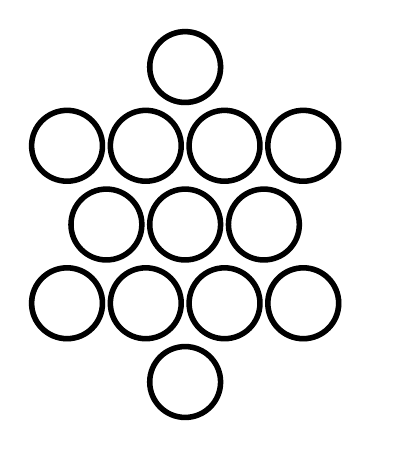
\begin{tikzpicture}[scale=0.5,line cap=round,line join=round,>=triangle 45,x=1.0cm,y=1.0cm]
      \clip(0,-1) rectangle (9,9);
      \alt<2->{\draw [line width=2.pt,color=lightgray] (1,2) circle (0.9cm);}
              {\draw [line width=2.pt] (1,2) circle (0.9cm);}
      \draw [line width=2.pt] (3,2) circle (0.9cm);
      \draw [line width=2.pt] (5,2) circle (0.9cm);
      \alt<3->{\draw [line width=2.pt,color=lightgray] (7,2) circle (0.9cm);}
              {\draw [line width=2.pt] (7,2) circle (0.9cm);}
      \draw [line width=2.pt] (2,4) circle (0.9cm);
      \draw [line width=2.pt] (4,4) circle (0.9cm);
      \draw [line width=2.pt] (6,4) circle (0.9cm);
      \draw [line width=2.pt] (3,6) circle (0.9cm);
      \draw [line width=2.pt] (5,6) circle (0.9cm);
      \alt<3->{\draw [line width=2.pt,color=lightgray] (4,8) circle (0.9cm);}
              {\draw [line width=2.pt] (4,8) circle (0.9cm);}
      \uncover<2->{\draw [line width=2.pt] (4,0) circle (0.9cm);}
      \uncover<3->{\draw [line width=2.pt] (7,6) circle (0.9cm);}
      \uncover<3->{\draw [line width=2.pt] (1,6) circle (0.9cm);}
    \end{tikzpicture}
  \end{center}
  Antwoord: \uncover<3->{De cirkels op de hoekpunten.}
\end{frame}

\begin{frame}
  \frametitle{Streepje plaatsen}
  \uncover<+->{
  Onderstaande gelijkheid klopt niet:
   \[\scalebox{1.2}{$5 + 5 + 5 = 550$}\]
   Hoe kan je de gelijkheid kloppend maken door slechts één streepje
   te zetten?  } \vfill \uncover<+->{ {\color{blue} Een hint: Een
     streepje door het gelijkheidsteken zetten is een originele
     oplossing, maar maakt een ongelijkheid van de gelijkheid en dat
     willen we niet!}  } \vfill Antwoord:
 \uncover<+->{\[\scalebox{1.2}{$5+5\;\;4\;\;5=550$}\]}
\end{frame}

\newcommand{\koffer}[2]{
  \begin{tikzpicture}[scale=0.9,line cap=round,line join=round,>=triangle 45,x=1.0cm,y=1.0cm]
    \clip(-0.1,-0.5) rectangle (3.6,2.);
    \draw [line width=1.6pt] (0.,0.)-- (2.5,0.);
    \draw [line width=1.6pt] (2.5,0.)-- (3.5,0.5);
    \draw [line width=1.6pt] (2.5,0.)-- (2.5,1.);
    \draw [line width=1.6pt] (2.5,1.)-- (3.5,1.5);
    \draw [line width=1.6pt] (3.5,1.5)-- (3.5,0.5);
    \draw [line width=1.6pt] (2.5,1.)-- (0.,1.);
    \draw [line width=1.6pt] (0.,1.)-- (0.,0.);
    \draw [shift={(3.15,0.94)},line width=1.6pt]
    plot[domain=1.01:3.06,variable=\t]
    ({1.*0.66*cos(\t r)+0.*0.66*sin(\t r)},{0.*0.66*cos(\t r)+1.*0.66*sin(\t r)});
    \draw [line width=2.pt] (0.60,1.60)-- (3.10,1.60);
    \draw [shift={(0.65,0.94)},line width=1.6pt]
    plot[domain=1.65:3.06,variable=\t]
    ({1.*0.66*cos(\t r)+0.*0.66*sin(\t r)},{0.*0.66*cos(\t r)+1.*0.66*sin(\t r)});
    \draw (2.7,1) node[anchor=north west] {\bf#1};
    \draw (-.1,1) node[anchor=north west] {\scriptsize\begin{tabular}{c}#2\end{tabular}};
  \end{tikzpicture}
}

\begin{frame}
  \frametitle{Optellen en vermenigvuldigen}
  Welke 3 strikt positieve gehele getallen geven hetzelfde resultaat als we ze optellen of als we ze vermenigvuldigen?
  \vfill
  \begin{align*}
    a + b + c &= z\\
    a \times b \times c &= z
  \end{align*}
  \begin{align*}
    \uncover<3->{1 + 2 + 3} &= \uncover<2->{6}\\
    \uncover<3->{1 \times 2 \times 3} &= \uncover<2->{6}
  \end{align*}
  \vfill
  Antwoord: \uncover<3->{1, 2 en 3}
\end{frame}

\begin{frame}
  \frametitle{Zoek het goud}
  Er zit goud in precies één koffer en op precies één koffer staat een
  ware uitspraak. Waar zit het goud?
  \vfill
  \begin{changemargin}{-1.cm}{-0.5cm}
    \begin{multicols}{4}
      \begin{center}
        \koffer{1}{Het goud zit\\ in koffer 2}
        \koffer{2}{Alle andere\\ koffers zijn leeg}
        \koffer{3}{Deze koffer\\ bevat het goud}
        \koffer{4}{Deze koffer\\ is leeg}
      \end{center}
    \end{multicols}
  \end{changemargin}
  \vfill
  Antwoord:
  \begin{itemize}
  \item<2-> het goud zit in koffer $1$
  \item<3-> de ware uitspraak staat op koffer $4$.
  \end{itemize}
\end{frame}


\begin{frame}
  \frametitle{Vul aan}
  Vul volgende rij aan, geef op zijn minst twee getallen:
  \begin{center}
    \scalebox{1.2}{$4,\; 6,\; 9,\; 13,\; 18,\; 24,\; ?,\; ?,\; \ldots$}
  \end{center}
  \vfill
  \begin{center}
    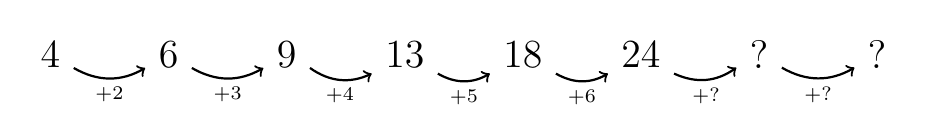
\begin{tikzpicture}
      [node distance = 1.5cm]
      \uncover<2->{
        \begin{Large}
          \node (4) {$4$};
          \node[right of = 4] (6) {$6$};
          \node[right of = 6] (9) {$9$};
          \node[right of = 9] (13) {$13$};
          \node[right of = 13] (18) {$18$};
          \node[right of = 18] (24) {$24$};
          \node[right of = 24] (31) {$?$};
          \node[right of = 31] (39) {$?$};
        \end{Large}
      }
      \begin{scriptsize}
        \uncover<3->{
          \draw[->, thick] (4) to[bend right=30] node[below] {$+2$} (6);
        }
        \uncover<4->{
          \draw[->, thick] (6) to[bend right=30] node[below] {$+3$} (9);
        }
        \uncover<5->{
          \draw[->, thick] (9) to[bend right=30] node[below] {$+4$} (13);
          \draw[->, thick] (13) to[bend right=30] node[below] {$+5$} (18);
          \draw[->, thick] (18) to[bend right=30] node[below] {$+6$} (24);
          \draw[->, thick] (24) to[bend right=30] node[below] {$+?$} (31);
          \draw[->, thick] (31) to[bend right=30] node[below] {$+?$} (39);
        }
      \end{scriptsize}
    \end{tikzpicture}
  \end{center}
  \vfill
  Antwoord:
  \uncover<5->{
    \begin{center}
      \scalebox{1.2}{$4,\; 6,\; 9,\; 13,\; 18,\; 24,\; 31,\; 39,\; \ldots$}
    \end{center}
  }
\end{frame}

\begin{frame}
  \frametitle{Associatieve}
  \scalebox{1.2}{$5 \times \left( 2 \times 9 \right)$} is ook gelijk aan

  \begin{enumerate}[(A)]
  \item $5-(2-9)$
  \item $5 \times 2-9$
  \item $( 5 \times 2 ) \times 9$
  \item $5 \times 10$
  \end{enumerate}
  \vfill
  \uncover<2->{
    $\mathbb{R},\times$ is {\bf associatief}, dit wil zeggen dat we haakjes mogen invoeren, verplaatsen of weglaten.
  }
  \vfill
  Antwoord: \uncover<3->{\quad (C)}\\
  \uncover<3->{
    \begin{center}
      \scalebox{1.2}{$5 \times \left( 2 \times 9 \right) = \left( 5
          \times 2 \right) \times 9$}
    \end{center}
  }
\end{frame}

\begin{frame}
  \frametitle{Aantal mogelijke uitslagen}
  Abel, Bernhard en Charlotte lopen om ter snelst de 100 m. Hoeveel
  mogelijke uitslagen zijn er?
%  \vfill
  \begin{center}
    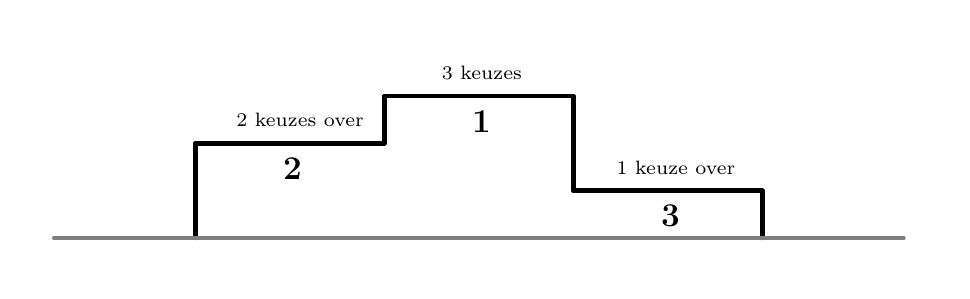
\begin{tikzpicture}[scale=0.3,line cap=round,line join=round,>=triangle 45,x=1.0cm,y=1.0cm]
      \clip(-7.1,-1.4) rectangle (31.6,8.9);
      \draw [line width=1.6pt] (0.,0.)-- (0.,4.);
      \draw [line width=1.6pt] (0.,4.)-- (8.,4.);
      \draw [line width=1.6pt] (8.,4.)-- (8.,6.);
      \draw [line width=1.6pt] (8.,6.)-- (16.,6.);
      \draw [line width=1.6pt] (16.,6.)-- (16.,2.);
      \draw [line width=1.6pt] (16.,2.)-- (24.,2.);
      \draw [line width=1.6pt] (24.,2.)-- (24.,0.);
      \draw [color=gray, line width=1.2pt] (-6.,0.)-- (30.,0.);
      \draw (11.3,5.8) node[anchor=north west] {\bf\large 1};
      \draw (3.3,3.8) node[anchor=north west] {\bf\large 2};
      \draw (19.3,1.8) node[anchor=north west] {\bf\large 3};
      \begin{scriptsize}
        \uncover<2->{\draw (10.1,7.6) node[anchor=north west] {$3$ keuzes};}
        \uncover<3->{\draw (1.4,5.6) node[anchor=north west] {$2$ keuzes over};}
        \uncover<4->{\draw (17.5,3.6) node[anchor=north west] {$1$ keuze over};}
      \end{scriptsize}
    \end{tikzpicture}
  \end{center}
  \vfill
  Antwoord: \quad $\uncover<6->{P_3= 3! = }\uncover<5->{3\cdot 2 \cdot 1 = 6}$
\end{frame}

\begin{frame}[fragile]
  \frametitle{Nobuyuki Yoshigahara (1936-2004)}
  \hfill Los Nob's nummer boom op!
  \vspace{-2em}
  \begin{center}
    \begin{dot2tex}[tikz, options=-tmath]
      digraph G {
        graph [ranksep=0.08, nodesep=0.5];
        node [shape=circle,fixedsize=true,width=0.3];
        edge [arrowhead=none]
        a [label="72"];
        b [label="99"];
        c [label="45"];
        d [label="39"];
        e [label="36"];
        f [label="28"];
        g [label="21"];
        12 [label="\alt<2>{12}{??}", style=filled, fillcolor="gray"];
        a -> 27 -> 18 -> 21 -> 12 -> 13 -> 7;
        b -> 27;
        c -> 18;
        d -> 21;
        e -> 12;
        f -> 13;
        g -> 7;
      }
    \end{dot2tex}
  \end{center}
  \vspace*{-2em}
  Antwoord: $\uncover<2->{2 + 1 + 3 + 6 = 12}$
\end{frame}

\newcommand{\rom}[1]{\uppercase\expandafter{\romannumeral #1\relax}}

\begin{frame} % bron: ppareit
  \frametitle{Stelsel}
  Gegeven:
  \begin{align*}
    \rom{5} + \rom{5} &= 10\\
    \rom{5} \times \rom{10} + \rom{10} &= 60\\
    \rom{10} - \rom{1} \times \rom{5} &= \rom{5}\\
  \end{align*}
  \vfill
  Bepaal: $$\rom{1} = \alt<1>{\;?}{1}$$

  \vfill
  Antwoord:
  \uncover<2->{
    \begin{align*}
      \rom{5} &= 5\\ \rom{10} &= 10\\ \rom{1} &= 1
    \end{align*}
  }
\end{frame}

\begin{frame}
  \frametitle{Einde}
  \vfill
  \begin{center}
    \Huge Goed gedaan!
  \end{center}
  \vfill
\end{frame}

\end{document}

% Local Variables:
% TeX-command-extra-options: "-shell-escape"
% End: